\documentclass{article}

\usepackage{fancyhdr}
\usepackage{extramarks}
\usepackage{amsmath}
\usepackage{amsthm}
\usepackage{amsfonts}
\usepackage{amssymb} % Equations
\usepackage{mathtools}
\usepackage{commath}
\usepackage{tikz}
\usepackage[plain]{algorithm}
\usepackage{algpseudocode}
\usepackage{adjustbox} % Used to constrain images to a maximum size 
\usepackage{xcolor} % Allow colors to be defined
\usepackage{enumerate} % Needed for markdown enumerations to work
\usepackage{geometry} % Used to adjust the document margins
\usepackage{textcomp} % defines textquotesingle
\usepackage[arrow,matrix,curve,cmtip,ps]{xy}
\usepackage{hyperref}

\usetikzlibrary{automata,positioning}

%
% Basic Document Settings
%

\topmargin=-0.45in
\evensidemargin=0in
\oddsidemargin=0in
\textwidth=6.5in
\textheight=9.0in
\headsep=0.25in

\linespread{1.1}

\pagestyle{fancy}
\lhead{\hmwkAuthorName}
\chead{\hmwkClass\ (\hmwkClassInstructor\ \hmwkClassTime): \hmwkTitle}
\rhead{\firstxmark}
\lfoot{\lastxmark}
\cfoot{\thepage}

\renewcommand\headrulewidth{0.4pt}
\renewcommand\footrulewidth{0.4pt}

\setlength\parindent{0pt}


%
% Create Problem Sections
%

\newcommand{\enterProblemHeader}[1]{
    \nobreak\extramarks{}{Problem \arabic{#1} continued on next page\ldots}\nobreak{}
    \nobreak\extramarks{Problem \arabic{#1} (continued)}{Problem \arabic{#1} continued on next page\ldots}\nobreak{}
}

\newcommand{\exitProblemHeader}[1]{
    \nobreak\extramarks{Problem \arabic{#1} (continued)}{Problem \arabic{#1} continued on next page\ldots}\nobreak{}
    \stepcounter{#1}
    \nobreak\extramarks{Problem \arabic{#1}}{}\nobreak{}
}

\setcounter{secnumdepth}{0}
\newcounter{partCounter}
\newcounter{homeworkProblemCounter}
\setcounter{homeworkProblemCounter}{1}
\nobreak\extramarks{Problem \arabic{homeworkProblemCounter}}{}\nobreak{}

%
% Homework Problem Environment
%
% This environment takes an optional argument. When given, it will adjust the
% problem counter. This is useful for when the problems given for your
% assignment aren't sequential. See the last 3 problems of this template for an
% example.
%
\newenvironment{homeworkProblem}[1][-1]{
    \ifnum#1>0
        \setcounter{homeworkProblemCounter}{#1}
    \fi
    \section{Problem \arabic{homeworkProblemCounter}}
    \setcounter{partCounter}{1}
    \enterProblemHeader{homeworkProblemCounter}
}{
    \exitProblemHeader{homeworkProblemCounter}
}

%
% Homework Details
%   - Title
%   - Due date
%   - Class
%   - Section/Time
%   - Instructor
%   - Author
%

\newcommand{\hmwkTitle}{Homework 03}
\newcommand{\hmwkDueDate}{Oct 11, 2018}
\newcommand{\hmwkClass}{Math 6366 Optimization}
\newcommand{\hmwkClassTime}{}
\newcommand{\hmwkClassInstructor}{Andreas Mang}
\newcommand{\hmwkAuthorName}{\textbf{Jonathan Schuba}}

%
% Title Page
%

\title{
    \textmd{\textbf{\hmwkClass:\ \hmwkTitle}}\\
    \normalsize\vspace{0.1in}\small{Due\ on\ \hmwkDueDate}\\
}
\author{\hmwkAuthorName}
\date{}

\renewcommand{\part}[1]{\textbf{\large Part \Alph{partCounter}}\stepcounter{partCounter}\\}

%
% Various Helper Commands
%

% Useful for algorithms
\newcommand{\alg}[1]{\textsc{\bfseries \footnotesize #1}}
% For derivatives
\newcommand{\deriv}[1]{\frac{\mathrm{d}}{\mathrm{d}x} (#1)}
% For partial derivatives
\newcommand{\pderiv}[2]{\frac{\partial}{\partial #1} (#2)}
% Integral dx
\newcommand{\dx}{\mathrm{d}x}
% Alias for the Solution section header
\newcommand{\solution}{\textbf{\large Solution}}


%-------------------------------------------
%       Begin Local Macros
%-------------------------------------------
\newcommand{\Gal}{\mathrm{Gal}}
\newcommand{\Aut}{\mathrm{Aut}}
\newcommand{\Prob}{\mathbf{P}}
\newcommand{\Pow}{\mathcal{P}}
\newcommand{\F}{\mathcal{F}}
\newcommand{\M}{\mathcal{M}}
\newcommand{\A}{\mathcal{A}}
\newcommand{\B}{\mathcal{B}}
\newcommand{\E}{\mathcal{E}}
\newcommand{\n}{\noindent}
\newcommand{\Z}{\mathbb{Z}}
\newcommand{\N}{\mathbb{N}}
\newcommand{\Q}{\mathbb{Q}}
\newcommand{\R}{\mathbb{R}}
\newcommand{\C}{\mathbb{C}}
\newcommand{\T}{\mathbb{T}}
\newcommand{\im}{\operatorname{im}}
\newcommand{\coker}{\operatorname{coker}}
\newcommand{\ind}{\operatorname{ind}}
\newcommand{\rank}{\operatorname{rank}}
\newcommand\mc[1]{\marginpar{\sloppy\protect\footnotesize #1}}
\newcommand{\ra}{\rangle}
\newcommand{\la}{\langle}
%-------------------------------------------
%       end local macros
%-------------------------------------------




\begin{document}

\maketitle

\begin{homeworkProblem}[1]
	Consider the optimization problem
	\[
	\begin{aligned}
		\underset{x\in\R^2}{\text{minimize}} \quad & f_0(x) \\ 
		\text{subject to} \quad & 2x_1+x_2\ge 1 \\ 
		& x_1+3x_2\ge 1 \\ 
		& x_1 \ge 0 \\ 
		& x_2 \ge 0
	\end{aligned} 
	\]
	Make a sketch of the feasible set. 
	
	\begin{figure}[h]
		\centering
		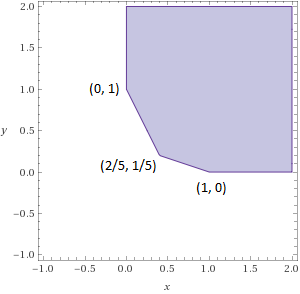
\includegraphics[width=0.4\linewidth]{image/q01}
		\caption{}
		\label{fig:q01}
	\end{figure}

		
	For each of the following objective functions, give the optimal set and
	the optimal value.
	\begin{enumerate}[a]
		\item $f_0(x) = x_1 + x_2$.
		\subitem {The optimal point is $(2/5, 1/5)$ and the optimal value is $3/5$.}
		
		\item $f_0(x) = \max \{x_1,x_2\}$.
		\subitem { The optimal point is $(1/3, 1/3)$ and the optimal value is $1/3$. }
		
		\item $f_0(x) = x_1^2 + 9x_2^2$.
		\subitem {The optimal point is $(1/2, 1/6)$ and the optimal value is $1/2$.}
		
	\end{enumerate}

	
\end{homeworkProblem}

\begin{homeworkProblem}[2]
	Verify that $x^* = \begin{bmatrix}1 \\	0.5 \\ 	-1	\end{bmatrix} $ is optimal for the optimization problem
	\[
	\begin{aligned}
	\underset{x\in\R^3}{\text{minimize}} \quad & \frac{1}{2}x^\top A x +q^\top x + r \\
	\text{subject to} \quad & -1 \le x_i \le 1, i = 1,2,3
	\end{aligned}
	\]

	where $A = \begin{bmatrix}
	13& 12& -2 \\ 12& 17& 6 \\ -2& 6& 12	
	\end{bmatrix}$ , $q = \begin{bmatrix}
	-22 \\ -14.5 \\ 30
	\end{bmatrix}$ and $r = 1$.
	
	This is a quadratic, convex objective, so the optimal value occurs when the gradient is zero.
	
	\[ \nabla f_0(x) = Ax + q^\top = 0 \]
	\[
	\nabla f_0(x^*) = \begin{bmatrix}
	13& 12& -2 \\ 12& 17& 6 \\ -2& 6& 12	
	\end{bmatrix} * x^* + \begin{bmatrix}
	-22 \\ -14.5 \\ 30
	\end{bmatrix}^\top = \begin{bmatrix}-1 \\	0 \\ 	19	\end{bmatrix}
	\]
	So, at $x^*$, the gradient is not zero in all directions.  But the objective value only gets better for increasing $x_1$ and decreasing $x_3$, which would put us outside of the constraints.  The gradient for $x_2$ is zero, so the value of $x_2$ is optimal here. 
	
	
\end{homeworkProblem}

\begin{homeworkProblem}[3]
	content...
\end{homeworkProblem}



\end{document}
